\chapter{Soluzione proposta}
L'approccio vincente si è basato su \textbf{locality-sensitive hashing} (LSH).
Gli approcci basati su LSH consistono nella definizione di una funzione di hash 
che ha l'obiettivo di partizionare il dataset $D$ in una hash table composta 
da una serie di bucket, ciascuno 
formato in modo tale da contenere vettori che sono i più simili possibili, rispetto 
alla distanza euclidea. 

La costruzione della funzione di hash deve essere fatta in modo tale da 
massimizzare il numero di collisioni tra i vettori simili e ridurre al minimo 
il numero di collisioni per vettori differenti. 

In questo modo la ricerca si articola in:
\begin{itemize}
    \item calcolare l'hash della query che definisce l'indice del bucket
    \item calcolare le distanze tra la query e tutti i vettori nel bucket ed 
    estrarre i 100 più vicini
\end{itemize} 

Questo approccio permette di ridurre il numero di distanze calcolate, dal momento 
che si confrontano solo la query con i vettori nel bucket. Il problema è trovare 
un approccio per costruire una funzione di hash che sia veloce da calcolare e 
che permetta di creare dei bucket di buona qualità.

\section{Costruzione della funzione di hash}

La funzione di hash che è stata definita si basa su \textbf{Random Projection}(RP),
esattamente lo stesso algoritmo di riduzione di dimensionalità. 

L'idea è di definire $k' = \lceil \log_2{\sqrt{|D|}} + 2\rceil (= 14)$  iperpiani randomici che suddividono
lo spazio dei vettori del dataset in $2^{k'}$ regioni, ad ogni regione si associa 
un hash e tutti i vettori che cadono afferiscono alla stessa regione produrranno 
una collisione, quindi verranno inseriti nello stesso bucket.

\begin{nota}
    La formula per ottenere $k'$ è stata scelta in modo arbitrario basandosi sulle 
    sugli studi empirici e suoi risultati ottenuti in termini di Recall e tempi
    di esecuzione.
\end{nota}

Ogni singolo $i$-esimo iperpiano è stato definito dal suo vettore norma $n_i$,
generato randomicamente estraendo le singole componenti da una distribuzione uniforme 
($n_i \in U[-1,1]^{100}$). L'hash di un vettore viene calcolato considerandolo 
come un numero binario di $k'$ bit, dove l'$i$-esimo bit $h_i$ dell'hash specifica:
\begin{itemize}
    \item $h_i = 1$: il vettore $v$ si trova sopra L'iperpiano definito dalla 
    norma $n_i$
    \item $h_i = 0$: il vettore $v$ si trova sotto L'iperpiano definito dalla 
    norma $n_i$
\end{itemize}

A livello matematico si riduce all'equazione 
$$h_i = \begin{cases}
    1 & n_i \cdot v \ge 0\\
    0 & n_i \cdot v < 0
\end{cases}$$ 

Dove $\cdot$ è il prodotto interno in $\mathbb{R}^{100}$. Lo pseudocodice della 
funzione di hash è stato riportato nel listato \ref{list:funzione_hash}.

\begin{algorithm}
    \SetAlgoLined
    \KwData{vettore $v\in D$}
    \KwResult{hash $h\in \mathbb{N}$}

    \Begin{
        $h= 0$\;
        \For{$i=1$ \KwTo $k'$}{
            $partial = n_i \cdot v$\;
            $h = h << 1$\;
            \If{$partial \ge 0$}{
                $h= h+1$\;
            }
        }
    }
    \caption{Pseudocodice della funzione di hash.}
    \label{list:funzione_hash}
\end{algorithm}

\begin{nota}
    L'hash viene calcolato solo sulle componenti del vettore e non sui metadati.
\end{nota}

La complessità temporale della funzione di hash calcolata per un particolare $v\in V$,
è $\mathcal{O}(k' \cdot |v|)$ dove 
$|v|$ è il numero delle componenti di $v\in D$ che dai requisiti della challenge 
costante a $100$, perciò si può anche approssimare a $\mathcal{O}(k')$, ma essendo 
che anche $k'$ è costante allora si piò approssimare a $\mathcal{O}(1)$.

\section{Costruzione di LSH}

La struttura dati di LSH dovrà contenere l'hash table dei vettori e le norme degli 
iperpiani generati.
Nella realtà viene salvato anche il mapping inverso dal vettore del dataset al 
suo hash associato.

La costruzione della struttura si articola in tre passi:
\begin{itemize}
    \item calcolo dell'hash per ogni vettore del dataset e salvataggio del mapping 
    vettore-hash
    \item creazione dei bucket e inserimento dei vettori
    \item ordinamento dei vettori nei bucket
\end{itemize}

Il calcolo dell'hash viene effettuato per ogni vettore e si salva il risultato 
all'interno di un array $v_h$:

$$v_h[i] = h(v_i)$$

Successivamente si costruiscono i bucket $M_h$, a livello implementativo ciascun bucket 
è una \texttt{unordered\_map}, che coincidono con 

$$M_h = \{v\in D : h = h(v)\}$$

\begin{nota}
    La scelta di utilizzare \texttt{unordered\_map} piuttosto che \texttt{map} è dovuta ai tempi di 
    accesso e ricerca degli elementi:
    \begin{itemize}
        \item \texttt{unordered\_map}: il tempo di accesso usando l'hash è costante 
        nel caso medio e lineare nel caso peggiore, inoltre il tempo di ottenimento dell'hash 
        dato un vettore è costante nel caso medio e lineare nel caso peggiore. \cite{unsorted_map_index}\cite{unsorted_map_find}
        \item \texttt{map}: il tempo di accesso usando l'hash è logaritmico nella dimensione 
        del container, mentre il tempo di ottenimento dell'hash dato un vettore è
        logaritmico. \cite{map_index}\cite{map_find}
    \end{itemize}
\end{nota}

Per ultimo si effettua un ordinamento dei vettori nei singoli bucket, più precisamente
si ordina prima timestamp e successivamente per le componenti dei vettori.

I tempi di costruzione della struttura coincidono con $\mathcal{O}(|D|\cdot 1)$
per il mapping vettore-hash, $\mathcal{O}(|D|\cdot |D|)$ ($\Theta(|D|)$) per l'inserimento 
dei vettori nei bucket e $\mathcal{O}(|D|\log |D|)$ per l'ordinamento dei vettori 

Parlando invece dello spazio occupato, la struttura ha una complessità spaziale 
limitata perché non si salvano completamente i vettori in ciascuna sottostuttura,
bensì si salvano i loro indici di posizione del dataset, in aggiunta gli hash non 
sono altro che interi. Quindi il vettore di mapping vettori-hash $v_h$ alla fine 
contiene un totale $|D|$ interi, mentre l'unsorted map conterrà sempre gli indici 
dei vettori, in totale $|D|$, e tutti gli hash, quindi al massimo $2^{k'} = 2^ {14}$ 
interi, infine complessivamente si ha un totale di al massimo $10^7 + 2^{14}$ interi 
da salvare ($\approx 38 Mb$).

Il problema di questa soluzione è la Recall che è risultata bassa fin da subito, 
in fatti uno dei problemi e allo stesso tempo pregi di questo metodo è che la ricerca 
dei vettori più vicini si effettua solo nel bucket in cui cade il vettore di query.
Questo permette di ridurre il numero di distanze calcolate per ogni query, ma non 
considera anche vettori vicini alla query che fanno parte di bucket adiacenti.

\begin{esempio}
    Se i dati sono molto densi in alcune regioni del piano e sparsi in altre c'\`e la possibilit\`a
    che un gruppo denso di punti sia diviso in pi\`u bucket limitando la nostra capacit\`a di leggere tutti
    i vettori "realmente" vicini a quello di query.
\end{esempio}

\begin{esempio}
    Possiamo aver problemi anche nel caso generale in cui la query sia di tipo $0$, quindi non si 
    deve filtrare per metadati, e cade nello spazio vicino ad un iperpiano che limita il bucket, 
    questo comporta che in fase di ricerca si consideranno solo i vettori di quel 
    bucket e non quelli del bucket adiacente che ha in comune lo stesso iperpiano. 
\end{esempio}

Per risolvere i problemi è stato pensato di generare nuovi mapping randomici (\textbf{LSH con hash table multiple})

\section{LSH con hash table multiple}

Precedentemente è stato introdotto LSH composta da una hash table che mappa i vettori 
in bucket identificati dal loro hash.

L'idea di LSH con hash table multiple è di creare un totale di $M$ hash table ognuna con un
inizializzazione tramite iperpiani il più differente possibile dalle altre. In questo 
modo è possibile suddividere l'intero spazio dei vettori in $M$ modi differenti,
cosicché in fase di ricerca, al posto che cercare in una hash table, si cerca 
in $M$ hash table parallelamente. In questo modo si può considerare anche alcuni vettori che ricadrebbero in bucket vicini,
perché si spera che i bucket in cui cade la query per ciascuna hash table siano composti da vettori diversi.
$M$ è stato scelto attraverso uno studio sull'impatto dei parametri sulle sulle metriche di tempo (di costruzione e ricerca) e recall.

La differenza di partizione dello spazio di ciascuna hash table dipende interamente 
da come vengono generati gli iperpiani di separazione, dal momento che si estraggono 
da una distribuzione uniforme si ha già una buona variabilità e questo permette di avere 
una maggior variabilità anche nelle hash table, portando a dei miglioramenti in termini di 
recall.

Bisogna però menzionare il fatto che le diverse hash table partizionano lo stesso 
spazio geometrico, quindi in fase di ricerca può capitare che la query venga confrontata 
più volte con gli stessi vettori perché questi, essendo vicini, possono capitare 
negli stessi bucket della query in hash table differenti.

Quindi introducendo $M$ hash table multiple, significa che si effettueranno $M$ 
diverse separazioni dello spazio dei vettori del dataset, perciò si avranno 
$M$ diversi insiemi di norme e perciò il calcolo dell'hash per ciascuna hash table 
si basa sull'insieme di norme associate alla medesima hash table.

Visto che l'introduzione di hash table multiple può portare a confronti multipli 
tra la query e gli stessi vettori, per ridurre i tempi di ricerca e aumentare 
la recall sulle query di tipo $1$ e di tipo $3$ è stato pensato di definire una 
\textbf{LSH Forest}.

\section{Esplorazione dei Bucket Adiacenti}

Si \`e anche pensato alla possibilit\`a di identificare a runtime i bucket adiacenti a quello della query per esplorarli e migliorare la recall, come alternativa ad avere pi\`u hash tables.
Questa operazione pu\`o essere fatta semplicemente considerando la \textbf{distanza di hamming} di due hash: con $HD = 1$ i due hash differiranno del posizionamento rispetto ad un iperpiano, di conseguenza esplorando tutti gli hash con questa distanzia stiamo visitando gli spazi adiacenti. Questo corrisponde ad effetturare uno xor dell'hash con $k$ bitmask del tipo $0^i10^j$, con $i + j + 1 = k$.
Il problema principale di questa strategia non \`e nella sua implementazione quanto nel fatto che rappresenta un'ennesima euristica basata sulla fortuna: se un query viene mappato in un bucket con pochi vettori e poi esplorando gli adiacenti ci imbattessimo in un bucket con molti vettori andremmo a peggiorare notevolmente l'esecuzione senza avere la certezza di trovare pi\`u vicini.
Sperimentalmente si \`e rilevato che l'aumento di recall \`e relativamente insignificante e che viceversa l'aumento dei tempi di ricerca peggiora nel complesso la qualit\`a della soluzione.

\section{LSH Forest}
L'approccio di LSH Forest è di velocizzare le query che filtrano sulla categoria,
ovvero quelle di tipo $1$ e $3$. Per fare ciò è stato pensato di definire una \textbf{LSH
con hash table multiple generale} sull'intero dataset per le query di tipo $0$ e $2$ e definire,
per ogni categoria sufficientemente grande ($>2000$), una \textbf{LSH con hash table multiple}, in questo 
modo si riduce il numero di distanze calcolate. La scelta di creare 
una LSH dedicata solo per le categorie che superano la cardinalità dei $2000$ vettori 
è dovuta dal fatto che il tempo necessario per crearla è maggiore dei benefici 
che porta nella ricerca, quindi si preferisce evitare di crearla.

L'unico problema che rimane da risolvere in fase di costruzione di LSH Forest è 
indentificare i vettori della stessa categoria nel dataset, per fare ciò è bastato 
ordinare il dataset dei vettori secondo la categoria, il timestamp ed infine 
le componenti di ciascun vettore. Questo richiede $\mathcal{O}(|D|\log |D|)$ di 
complessità, ma non aggiunge complessità alla costruzione delle LSH per ogni categoria 
dal momento che i vettori della stessa categoria sono tutti continui. Questa 
fase di ordinamento, inoltre, velocizza l'ordinamento dei vettori nei bucket e la ricerca 
filtrando per il timestamp. L'ordinamento dei vettori del bucket non è detto 
che venga preservato perché la costruzione è parallelizzata.

Quindi ricapitolando la costruzione si articola nelle seguenti fasi:
\begin{itemize}
    \item \textbf{ordinamento del dataset} secondo la categoria, timestamp e componenti dei vettori.
    \item \textbf{indicizzazione delle categorie}: creazione di una mappa che 
    associa a ciascuna categoria una tupla che specifica gli indici 
    del primo e dell'ultimo vettore nel dataset di quella categoria.
    \item \textbf{creazione di LSH con hash table multiple} sull'intero dataset.
    \item \textbf{creazione di una LSH con hash table multiple} per ogni categoria 
    di dimensione maggiore di $2000$ vettori.
\end{itemize}

L'algoritmo finale di costruzione di LSH Forest è mostrato nel listato \ref{list:costruzione_lsh_forest}.

\begin{algorithm} [!h]
    \SetAlgoLined
    \KwData{dataset $D$}
    \KwResult{LSH Forest $LSHF$}
    
    \Begin{
        $sort(D)$\;
        $c\_map = index(D)$\;
        $LSHF.general = createLsh(D,0,|D| - 1)$\;
        \For{$\forall c\in C$}{
            \If{$c\_map[c].end - c\_map[c].start > 2000$}{
                $lsh = createLsh(D,c\_map[c].start,c\_map[c].end)$\;
            }{
                $lsh = Null$\;
            }
            $LSHF.mapped[c] = lsh$\;
        }
    }

    
    \SetKwFunction{FLsh}{createLsh}
    \SetKwProg{Fn}{Function}{:}{}
    \Fn{\FLsh{$D$, $start\_idx\_cat$, $end\_idx\_cat$}}{
        \Begin{
            $lsh$ is object\;
            $length =end\_idx\_cat - start\_idx\_cat$\;
            \For{$i=1$ \KwTo $NHashTable$}{
                $hp = generateHyperplanes()$\;
                $lsh.hashtable[i].hp = hp$\;
                $hashes$ is array\;
                \For{$j=1$ \KwTo $|length|$}{
                    \For{$k=1$ \KwTo $|hp|$}{
                        $hashes[j] = hash(hp[k], D[start\_idx\_cat + j])$\;
                    }
                }
                $lsh.hashtable[i].hashes = hashes$\;
                \For{$j=1$ \KwTo $|D|$}{
                    $lsh.hashtable[i].buckets[hashes[j]].push(start\_idx\_cat + j)$\;
                }

                \For{$j=1$ \KwTo $|hp|$}{
                    $sort(lsh.hashtable[i].buckets[j])$\;
                }
            }
            \Return{$lsh$}
        }
    }

    \caption{Pseudocodice della costruzione di LSH Forest. La funzione $index$ genera 
    una mappa che associa ad ogni categoria la posizione di inizio e di fine del 
    gruppo di vettori che afferisce alla stessa categoria. La funzione 
    $generateHyperplanes$ ritorna l'array delle norme degli iperpiani generate 
    randomicamente.}
    \label{list:costruzione_lsh_forest}
\end{algorithm}

La complessità di creazione di LSH Forest può essere riassunta in:
\begin{itemize}
    \item \textbf{ordinamento del dataset}: $\mathcal{O}(|D|\log |D|)$
    \item \textbf{indicizzazione delle categorie}: $\mathcal{O}(|D|)$
    \item \textbf{creazione di LSH con hash table multiple} generale: la generazione
    di una hash table richiede $\mathcal{O}(k'\cdot |v|=1)$ per generare gli iperpiani
    (dove $|v| = 100, k' = 14$), $\mathcal{O}(|D|\cdot 1)$ per calcolare l'hash per ogni vettore,
    $\mathcal{O}(|D|)$ per inserire i vettori nei bucket e infine $\mathcal{O}(|D|\log |D|)$
    per ordinare tutti i bucket. Queste operazioni si devono replicare per tutte le 
    $M$ hash table quindi in totale si impiegherà $\mathcal{O}(M\cdot |D|\log |D|)$.
    Da notare che i bucket potenzialmente sono già parzialmente ordinati quindi 
    l'ordinamento a livello asintotico si avvicina a $\mathcal(|D|)$ e quindi 
    potenzialmente la complessità della creazione di tutte le hash table è $\mathcal{O}(M\cdot |D|)$.
    \item \textbf{creazione di una LSH con hash table multiple} per ogni categoria 
    di dimensione maggiore di $2000$ vettori: per la creazione di ciascuna LSH 
    è, come detto precedentemente, vicino a $\mathcal{O}(M\cdot |c|)$ dove $|c|$
    è la dimensione della categoria.
\end{itemize}

In realtà la costruzione viene ottimizzata parallelizzando la costruzione delle 
singole LSH.

\section{Ricerca in LSH Forest}

La ricerca nella struttura cambia in base alla tipologia di query che si deve 
cercare:
\begin{itemize}
    \item query senza filtraggio e query con il filtraggio sul timestamp: la ricerca 
    si effettua solo nell'LSH generale contenente tutti i vettori.
    \item query con il filtraggio sulla categoria e query con il filtraggio sulla 
    categoria e timestamp: la ricerca si effettua in modo esaustivo nel dataset per quelle 
    categorie con meno di $2000$ vettori, altrimenti per le altre si ricerca 
    nella LSH della categoria. 
\end{itemize}

Per ogni query si produce un Minheap contenente le $100$ migliori coppie 
$(idx_v, d(v,q))$, ovvero indice del vettore $v$ nel dataset e distanza tra il vettore
e la query. Il Minheap deve ordinare rispetto la distanza.

La ricerca di una \textbf{query senza filtraggio o query con filtraggio sul timestamp} 
si effettua nell'LSH generale costruita sull'intero dataset. Più precisamente la 
query senza filtraggio si ricerca nel seguente modo, per ogni hash table 
delle $20$ si estraggono i vettori a distanza minima dalla query e poi si combinano 
i risultati. Più precisamente, per ogni $i$-esima hash table:
\begin{itemize}
    \item si calcola $h_i(q)$
    \item si cerca il bucket di vettori che sono mappati con il medesimo hash 
    di $h_i(q)$
    \item si calcolano le distanze tra i vettori del bucket e la query e si inseriscono
    nel Minheap
\end{itemize}
Per il caso delle query con filtraggio sul timestamp si effettuano i seguenti passi,
per ogni $i$-esima hash table:
\begin{itemize}
    \item si calcola $h_i(q)$
    \item si cerca il bucket di vettori che sono mappati con il medesimo hash 
    di $h_i(q)$
    \item si effettua una ricerca dicotomica nel bucket degli indici di due vettori: quello con 
    il minimo timestamp che è maggiore di $q.l$ e quello col massimo timestamp che 
    è minore di $q.r$. In questo modo si trova il intervallo di vettori nel bucket 
    che hanno timestamp compreso tra $[l,r]$.
    \item si calcolano le distanze tra i vettori del bucket e la query e si inseriscono
    nel Minheap
\end{itemize}

La ricerca di una \textbf{query con filtraggio solo sulla categoria o sulla categoria e timestamp}, 
per categorie piccole $|c|\le 2000$, viene effettuata in modo esaustivo direttamente nel dataset,
sfruttando il suo ordinamento e l'indicizzazione della $c\_map$ costruita 
prima di creare $LSHForest$. 
Più precisamente, dal momento che il dataset viene ordinato, da $c\_map[c]$
si ottiene $[idx_l, idx_r]$, l'intervallo vettori afferenti alla stessa categoria della query. 
Se la query filtra solo per categoria si calcolano le distanze tra la query e tutti 
i vettori della regione, popolando di conseguenza il minheap. 
Nel caso in cui la query filtra anche per timestamp, 
dal momento che la regione è anche ordinata per timestamp, allora si effettua 
una ricerca dicotomica degli indici di due vettori: quello con il minimo timestamp che è 
maggiore di $q.l$ e quello col massimo timestamp che è minore di $q.r$.
In questo modo si ottiene un intervallo 
di indici dei vettori nel dataset che hanno timestamp incluso 
nell'intervallo specificato dalla query. Infine si calcolano tutte le distanze 
tra i vettori dell'intervallo e la query, popolando alla fine il minheap.

Per le medesime query, ma sulle categorie più grandi $|c|> 200$ allora la ricerca 
si effettua direttamente nelle LSH dedicate della categoria con lo stesso algoritmo 
spiegato per la ricerca delle query senza filtraggio o query con filtraggio sul timestamp.

Lo pseudocodice è mostrato nel listato \ref{list:ricerca_lsh_forest}.



\begin{algorithm} [!h]
    \SetAlgoLined
    \KwData{dataset $D$, $LSHF$ e query $q$}
    \KwResult{vettori $K \subseteq D$}
    
    \Begin{
        \Switch{query.type}{
            \Case{$query.type == 0 \lor query.type == 2$}{
                \Return{$searchLsh(LSHF.general, D, q)$}
            }
            \Case{$query.type == 1\lor query.type == 3$}{
                \If{$LSHF.mapped[c].hashtable != null$}{
                    \Return{$searchLsh(LSHF.mapped[c],D, q)$}
                }\Else{
                    \Return{$ExaustiveSearch(D, q)$}
                }
            }
        }
    }

    \SetKwFunction{FLsh}{searchLsh}
    \SetKwProg{Fn}{Function}{:}{}
    \Fn{\FLsh{$LSH$,$D$, $q$}}{
        \Begin{
            $results$ is a Minheap\;
            \Switch{$q.type$}{
                \Case{$q.type == 2 \lor q.type == 3$}{
                    \For{$i=1$ \KwTo $Ns$}{
                        $h_q = hash(LSH.hashtable[i],q)$\;
                        $bucket = LSH.hashtable[i].bucket[h_q]$\;
                        $[idx_l, idx_r] = dicotomicSearch(D, bucket, q.l, q.r)$\;

                        \For{$v\in D[idx_l:idx_r]$}{
                            \If{$\lnot results.has(v)$}{
                                $results.insert((idx(v), distance(v,q)))$\;
                            }                            
                        }
                        \Return{$lsh$}
                    }

                }
                \Case{$q.type == 0 \lor q.type == 1$}{
                    \For{$i=1$ \KwTo $NHashTable$}{
                        $h_q = hash(LSH.hashtable[i],q)$\;
                        $bucket = LSH.hashtable[i].bucket[h_q]$\;
                        $[idx_l, idx_r] = dicotomicSearch(D, bucket, q.l, q.r)$\;

                        \For{$idx\in bucket$}{
                            \If{$\lnot results.has(v)$}{
                                $results.insert((idx, distance(D[idx],q)))$\;
                            }              
                        }
                        \Return{$lsh$}
                    }

                }
            }
            
        }
    }

    \caption{Pseudocodice per la ricerca della query in LSH Forest.}
    \label{list:ricerca_lsh_forest}
\end{algorithm}

La complessità della ricerca varia in base alle query che si devono cercare e dalla 
composizione del dataset:
\begin{itemize}
    \item \textbf{query senza filtraggio}: il calcolo dell'hash è approssimato a $\mathcal{O}(1)$,
    trovare il bucket con lo stesso hash è $\mathcal{O}(|D|)$ (costante nel caso medio) e 
    si calcolano un totale di $\mathcal{O}(|b|)$ ($|b|$ numero di vettori nel bucket). 
    Questo ripetutto per tutte le $20$ che a livello asintotico rimane $\mathcal{O}(|D|)$
    o nel caso medio $\Theta(|b|)$.
    \item \textbf{query con filtraggio sul timestamp}: il calcolo dell'hash è approssimato a $\mathcal{O}(1)$,
    trovare il bucket con lo stesso hash è $\mathcal{O}(|D|)$ (costante nel caso medio),
    ricerca dicotomica dei due vettori nel bucket $\mathcal{O}(\log(|b|))$ ($|b|$ numero di vettori nel bucket) 
    e, supponendo che l'intervallo di timestamp sia grande $|t|\le |b|$ vettori, 
    si calcolano un totale di $\mathcal{O}(|t|)$. 
    Questo ripetuto per tutte le $20$ che a livello asintotico rimane $\mathcal{O}(|D|)$
    o nel caso medio $\Theta(|t|)$.
    \item \textbf{query con filtraggio solo sulla categoria} (categoria piccola): 
    si calcolano al massimo $\mathcal{O}(|c|)$ distanze, dove $|c|$ indica la dimensione 
    della categoria che per definizione sono $|c|\le 2000$.
    \item \textbf{query con filtraggio solo sulla categoria e sul timestamp} (categoria piccola): 
    si calcolano al massimo $\mathcal{O}(|t|)$ distanze, dove $|t|$ è il numero 
    di vettori che hanno timestamp incluso nell'intervallo specificato dalla query,
    nel caso peggiore $|t|=|c|$. 
    \item \textbf{query con filtraggio solo sulla categoria} (categoria grande):
    il calcolo dell'hash è approssimato a $\mathcal{O}(1)$,
    trovare il bucket con lo stesso hash è $\mathcal{O}(|c|)$ (costante nel caso medio), con
    $|c|$ dimensione della categoria, e 
    si calcolano un totale di $\mathcal{O}(|b|)$ ($|b|$ numero di vettori nel bucket).
    Questo ripetuto per tutte le $20$ che a livello asintotico rimane $\mathcal{O}(|c|)$
    o nel caso medio $\Theta(|b|)$.
    \item \textbf{query con filtraggio solo sulla categoria e sul timestamp} (categoria grande): 
    il calcolo dell'hash è approssimato a $\mathcal{O}(1)$,
    trovare il bucket con lo stesso hash è $\mathcal{O}(|c|)$ (costante nel caso medio), con
    $|c|$ dimensione della categoria, 
    ricerca dicotomica dei due vettori nel bucket $\mathcal{O}(\log(|b|))$ ($|b|$ numero di vettori nel bucket) 
    e, supponendo che l'intervallo di timestamp sia grande $|t|\le |b|$ vettori, 
    si calcolano un totale di $\mathcal{O}(|t|)$.
\end{itemize}

La complessità di costruzione della soluzione, ovvero il riempimento del minheap,
varia sempre in base alla categoria perché dipende interamente da quante distanze 
sono state calcolate. Supponendo che per una generica query vengono calcolate un 
totale di $d$ distanze, allora l'inserimento è $\mathcal{O}(d\cdot |MinHeap|)$, non è 
$\mathcal{O}(d\cdot \log(|MinHeap|))$ perché il minheap viene genestito con un vettore dal 
momento che la sua dimensione è limitata a $100$.

La complessità viene attenuata parallelizzando la ricerca nella varie LSH e hash table.

\section{Sensitività dei parametri}
Gli unici parametri dell'LSH Forest sono:
\begin{itemize}
    \item \textbf{LSH\_TABLES}: numero di hash table per la singola LSH.
    \item \textbf{LSH\_FOREST\_THRESHOLD}: numero massimo della dimensione della categoria per la
    quale non si crea la LSH dedicata.
\end{itemize} 

Quindi è stato necessario valutare come variano i tempi di esecuzione e la recall
al variare dei parametri. Di conseguenza è stato pensato di lanciare diverse 
esecuzioni di LSH Forest sul dataset d'esempio di $10^7$ vettori e limitando la ricerca delle query alle 
prime $4000$. Ciascuna esecuzione è stata lanciata con i seguenti intervalli di valori.
\begin{equation}
    \begin{array}{c}
        LSH\_TABLES \in \{1, 5, 10, 15, 20, 25, 30, 35\}\\
        LSH\_FOREST\_THRESHOLD \in \{0, 500, 1000, 2000, 5000, 7000, 10000, 15000\}
    \end{array}
\end{equation}

Per ogni esecuzione sono state salvate le seguenti metriche:
\begin{itemize}
    \item \textbf{build time}: tempo di costruzione della LSH generica sull'interno 
    dataset. le LSH dedicate per categoria sono state ignorate dal momento che il tempo maggiore nella costruzione 
    dipende da quella generale. Di conseguenza non si potrà visualizzare la variazione 
    del tempo di costruzione dell'LSH Forest in base al numero di LSH.
    \item \textbf{run time}: tempo di ricerca delle $4000$ query nella struttura.
    \item \textbf{recall}: confronto della soluzione ottenuta dalla ricerca con 
    la soluzioen dell'algoritmo esaustivo.
\end{itemize}

I risultati sono stati rappresentati all'interno di un grafico visibile nella figura 
\ref{fig:sensitivity}.

La prima osservazione che si evince dai grafici è che il parametro più significativo è LSH\_TABLES,
infatti più hash tables sono presenti in una LSH, maggiore è il tempo di costruzione 
e il run time con un conseguente aumento della recall, in accordo con quanto detto
e auspicato in precedenza.

LSH\_FOREST\_THRESHOLD non impatta significativamente nella recall 
ma, bensì, impatta maggiormente sulla memoria, aspetto che non è stato curato dal 
momento che non sono stati rilevati problemi di saturazione.

\begin{figure}[!h]
    \centering
    \begin{subfigure}{.5\textwidth}
      \centering
      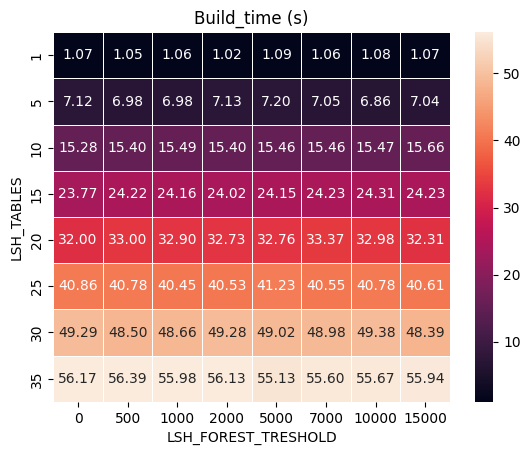
\includegraphics[width=.8\linewidth]{img/build_time.png}
      \caption{Building time della LSH generale}
      \label{fig:build_time}
    \end{subfigure}%
    \begin{subfigure}{.5\textwidth}
      \centering
      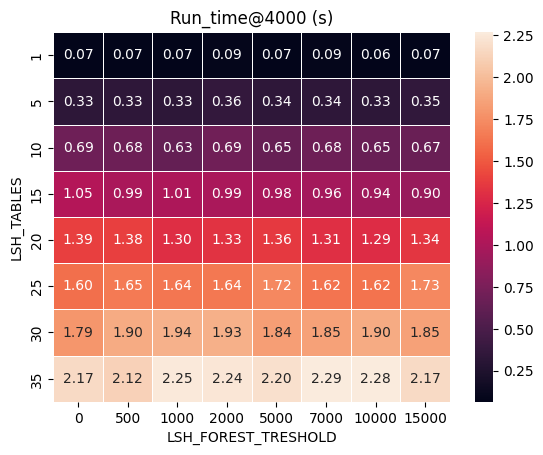
\includegraphics[width=.8\linewidth]{img/run_time.png}
      \caption{Run time}
      \label{fig:run_time}
    \end{subfigure}
    \begin{subfigure}{.5\textwidth}
      \centering
      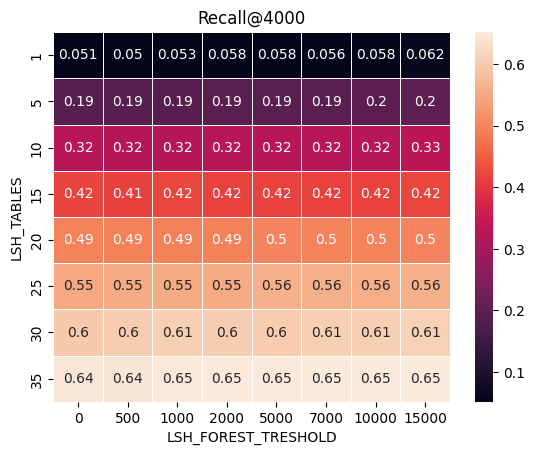
\includegraphics[width=.8\linewidth]{img/recall.png}
      \caption{Recall@4000}
      \label{fig:recall}
    \end{subfigure}
    \caption{Analisi di sensitività dei parametri, i tempi di costruzione non 
    variano al variare di LSH\_FOREST\_THRESHOLD dal momento che viene solo tracciato 
    il tempo di costruzione della LSH generale.}
    \label{fig:sensitivity}
\end{figure}

Dal momento che la Recall e il run time non vengono impattate notevolmente dal
parametro LSH\_FOREST\_THRESHOLD, risulta insignificativo evitare di creare una 
LSH dedicata per categoria. Nella soluzione consegnata è stato settato il 
parametro a $2000$.

Al contrario il parametro LSH\_TABLES è stato deciso in base ai vincoli di tempo 
richiesti dalla challenge, è stato scelto il valore $20$, ovvero il valore con la 
recall maggiore che permettesse di rispettare i vincoli di tempo. 




\section{Considerazioni}
LSH Forest è stato l'unico metodo che ci ha permesso di produrre una soluzione 
conforme ai limiti di $20$ minuti della challenge con recall maggiore rispetto
agli altri metodi ($\sim 0.4983$ sulla piattaforma di consegna). 

La motivazione per cui la recall è così bassa è dovuta principalmente dalla suddivisione 
dello spazio geometrico e dalla ricerca. Attualmente si effettuano $20$ suddisioni
dello spazio che non sono sufficientemente differenti, questo significa che in 
fase di ricerca, i bucket di ogni suddivisione in cui cade la query non hanno molta 
variabilità.

Si potrebbe migliorare questo aspetto andando cambiare il metodo di generazione 
degli iperpiani, in modo tale che ogni suddivisione dello spazio sia il più differente 
possibile, permettendo quindi di esplorare uno spazio più ampio di vettori 
sempre idealmente vicini alla query e riducendo il calcolo di distanze 
calcolate già in altre suddivisioni. 
